\documentclass[12pt]{article}


% ----------------- PAQUETES -----------------
\usepackage[utf8]{inputenc}
\usepackage[spanish]{babel}
\usepackage[margin = 2.54cm]{geometry}
\usepackage{graphicx}
\usepackage{enumitem}
\usepackage{parskip}
\usepackage{bm}
\usepackage[x11names,table]{xcolor}
\usepackage{amsmath}



% ----------------- CONFIGURACIONES -----------------
% ----------------- UTILIDADES PARA DAR UN MEJOR FORMATO DE DOCUMENTO -----------------  


\definecolor{azul}{rgb}{0.0039, 0.3098, 0.6196}


% Formato para el indice general ...........
\makeatletter
    \renewcommand{\@dotsep}{1.5}
    \renewcommand{\l@section}{\@dottedtocline{1}{1.5em}{2.3em}}
    \renewcommand{\l@subsection}{\@dottedtocline{2}{3.8em}{3.2em}}
    \renewcommand{\l@subsubsection}{\@dottedtocline{3}{7.0em}{4.1em}}
\makeatother

% --------- COMANDOS PERSONALIZADOS PARA LA PORTADA DE LAS TAREAS, TRABAJOS Y PROYECTOS ---------

\newcommand{\rutaLogo}[1]{\newcommand{\RutaLogo}{#1}}
\newcommand{\tema}[1]{\newcommand{\Tema}{#1}}
\newcommand{\etiquetaAutores}[1]{\newcommand{\EtiquetaAutores}{#1}}
\newcommand{\alumno}[1]{\newcommand{\Alumno}{#1}}
\newcommand{\materia}[1]{\newcommand{\Materia}{#1}}
\newcommand{\docente}[1]{\newcommand{\Docente}{#1}}
\newcommand{\ciclo}[1]{\newcommand{\Ciclo}{#1}}
\newcommand{\fecha}[1]{\newcommand{\Fecha}{#1}}
\newcommand{\periodo}[1]{\newcommand{\Periodo}{#1}}

\definecolor{celeste}{HTML}{94E4F1}


% ----------------- PORTADA -----------------
\rutaLogo{../../../docs/img/logo-ista.png}
\tema{\\ \vspace{0.8cm} Taller de ejercicios - Límites \\ \vspace{1.5cm}}
\etiquetaAutores{Alumno: }
\alumno{Eduardo Mendieta \vspace{0.8cm}}
\materia{Matemática \vspace{0.8cm}}
\docente{Lcda. Vilma Duchi, Mgtr. \vspace{0.8cm}}
\ciclo{Primer ciclo \vspace{0.8cm}}
\fecha{05/08/2024 \vspace{0.8cm}}
\periodo{Abril 2024 - Agosto 2024}


\begin{document}
    \begin{titlepage}

    \centering

    \includegraphics[width=0.11\textwidth]{\RutaLogo} 

    \vspace{0.3cm}
    \textcolor{azul}{\Large \textbf{Instituto Superior Universitario Tecnológico del Azuay \\}}
    \vspace{0.3cm}
    \textcolor{azul}{\Large \textbf{Tecnología Superior en Big Data}}
    
    % 1. ---------------- TEMA -------------------------
    
    {\Large\textbf{\Tema}}
    
    % 2. ---------------- AUTOR(ES) -------------------------
    \textcolor{azul}{\large \textbf{\EtiquetaAutores} \\}
    \vspace{0.3cm}
    {\large \Alumno}

    % 3. ---------------- MATERIA -------------------------
    \textcolor{azul}{\large \textbf{Materia:} \\}
    \vspace{0.3cm}
    {\large \Materia}


    % 3. ---------------- DOCENTE -------------------------
    \textcolor{azul}{\large \textbf{Docente:} \\}
    \vspace{0.3cm}
    {\large \Docente}


    % 3. ---------------- Ciclo -------------------------
    \textcolor{azul}{\large \textbf{Ciclo:} \\}
    \vspace{0.3cm}
    {\large \Ciclo}


    % 3. ---------------- FECHA -------------------------
    \textcolor{azul}{\large \textbf{Fecha:} \\}
    \vspace{0.3cm}
    {\large \Fecha}

    % 3. ---------------- PERIODO -------------------------
    \textcolor{azul}{\large \textbf{Periodo Académico:} \\}
    \vspace{0.3cm}
    {\large \Periodo}
 
\end{titlepage}


    \section*{\centering Taller de ejercicios - Límites}
        \textbf{Resolver los siguientes ejercicios:}

        \begin{enumerate}
            % EJERCICIO 1: ---------------------------------------------------
            \item Estime el valor del límite haciendo una tabla de valores, compruebe su trabajo con una gráfica:
                \begin{enumerate}[label=\textbf{\arabic*)}] 
                    \item \[\bm{\lim_{x \to 5} \frac{x ^2 - 25}{x - 5}}\]
                    \item \[\bm{\lim_{x \to 3} \frac{x ^2 - x - 6}{x - 3}}\]
                \end{enumerate}


            % EJERCICIO 2: ---------------------------------------------------
            \item Complete la tabla de valores (a cinco lugares decimales), y use la tabla para estimar el valor del límite:
                \begin{enumerate}[label=\textbf{\arabic*)}] 
                    \item \[\bm{\lim_{x \to 4} \frac{\sqrt{x} - 2}{x - 4}}\]
                        \begin{table}[h]
                            \centering
                            \begin{tabular}{|>{\columncolor{celeste}}l|l|l|l|l|l|l|l|l|l|l|l|}
                                \hline
                                $\bm{x}$ & 3.9 & 3.99 & 3.999 & 3.9999 & 3.99999 & \textbf{4} & 4.00001 & 4.0001 & 4.001 & 4.01 & 4.1 \\
                                \hline
                                $\bm{f(x)}$ &  &  &  &  &  &  &  &  &  &  &  \\
                                \hline
                            \end{tabular}
                        \end{table}


                    \item \[\bm{\lim_{x \to 2} \frac{x - 2}{x ^2 + x - 6}}\]
                        \begin{table}[h]
                            \centering
                            \begin{tabular}{|>{\columncolor{celeste}}l|l|l|l|l|l|l|l|l|l|l|l|}
                                \hline
                                $\bm{x}$ & 1.9 & 1.99 & 1.999 & 1.9999 & 1.99999 & \textbf{2} & 2.00001 & 2.0001 & 2.001 & 2.01 & 2.1 \\
                                \hline
                                $\bm{f(x)}$ &  &  &  &  &  &  &  &  &  &  &  \\
                                \hline
                            \end{tabular}
                        \end{table}
                        

                    \item \[\bm{\lim_{x \to 1} \frac{x - 1}{x ^3 - 1}}\]
                        \begin{table}[h]
                            \centering
                            \begin{tabular}{|>{\columncolor{celeste}}l|l|l|l|l|l|l|l|l|l|l|l|}
                                \hline
                                $\bm{x}$ & 0.9 & 0.99 & 0.999 & 0.9999 & 0.99999 & \textbf{1} & 1.00001 & 1.0001 & 1.001 & 1.01 & 1.1 \\
                                \hline
                                $\bm{f(x)}$ &  &  &  &  &  &  &  &  &  &  &  \\
                                \hline
                            \end{tabular}
                        \end{table}

                \end{enumerate}
            
            % EJERCICIO 3: ---------------------------------------------------
            \newpage
            \item Para la función $f$ cuya gráfica nos dan, exprese el valor de la cantidad dada si existe; si no existe, explique por qué:
                \begin{figure}[h!]
                    \centering
                    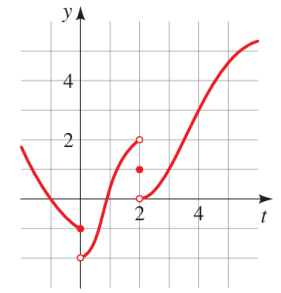
\includegraphics[width=0.4\textwidth]{img/t1-ej3.png}
                \end{figure}
            
                \begin{enumerate}[label=\textbf{\alph*.}]
                    \item \[\bm{\lim_{t \to 0 ^-} g(t)}\]
                    \item \[\bm{\lim_{t \to 0 ^+} g(t)}\]
                    \item \[\bm{\lim_{t \to 0} g(t)}\]
                    \item \[\bm{\lim_{t \to 2 ^-} g(t)}\]
                    \item \[\bm{\lim_{t \to 2 ^+} g(t)}\]
                    \item \[\bm{\lim_{t \to 2} g(t)}\]
                    \item \[\bm{g(2)}\]
                    \item \[\bm{\lim_{t \to 4} g(t)}\]
                \end{enumerate}
            
            % EJERCICIO 4: ---------------------------------------------------
            \item Use la tabla de valores para estimar el valor del límite. A continuación, use una calculadora gráfica para confirmar gráficamente sus resultados:
                \begin{enumerate}[label=\textbf{\arabic*)}] 
                    \item \[\bm{\lim_{x \to -4} \frac{x + 4}{x ^2 + 7x + 12}}\]
                    \item \[\bm{\lim_{x \to 1} \frac{x ^3 - 1}{x ^2 - 1}}\]
                    \item \[\bm{\lim_{x \to 0} \frac{5 ^x - 3^x }{x}}\]
                    \item \[\bm{\lim_{x \to 0} \frac{\sqrt{x + 9} - 3}{x}}\]
                \end{enumerate}

            
            % EJERCICIO 5: ---------------------------------------------------
            \item Evalúe el límite y justifique cada paso al indicar las leyes de límites apropiadas:
                \begin{enumerate}[label=\textbf{\arabic*)}] 
                    \item \[\bm{\lim_{x \to 4} (5x ^2 - 2x + 3)}\]
                    \item \[\bm{\lim_{x \to 3} (x ^3 + 2)(x ^2 - 5x)}\]
                    \item \[\bm{\lim_{x \to -1} \frac{x - 2 }{x ^2 + 4x - 3}}\]
                    \item \[\bm{\lim_{x \to 1} \left(\frac{x^4 + x^2 - 6}{x^4 + 2x + 3}\right)^2}\]
                \end{enumerate}

            
            % EJERCICIO 6: ---------------------------------------------------
            \item Evalúe el límite si existe:
                \begin{enumerate}[label=\textbf{\arabic*)}] 
                    \item \[\bm{\lim_{x \to 2} \frac{x ^2 + x - 6}{x - 2}}\]
                    \item \[\bm{\lim_{x \to -4} \frac{x ^2 + 5x +4}{x ^2 + 3x - 4}}\]
                    \item \[\bm{\lim_{x \to 2} \frac{x ^2 - x + 6}{x + 2}}\]
                    \item \[\bm{\lim_{x \to 1} \frac{x ^3 - 1}{x ^2 - 1}}\]
                    \item \[\bm{\lim_{t \to -3} \frac{t ^2 - 9}{2t ^2 + 7t + 3}}\]
                    \item \[\bm{\lim_{h \to 0} \frac{\sqrt{1 + h} - 1}{h}}\]
                    \item \[\bm{\lim_{h \to 0} \frac{(2 + h) ^3 - 8}{h}}\]
                    \item \[\bm{\lim_{x \to 2} \frac{x ^4 - 16}{x - 2}}\]
                    \item \[\bm{\lim_{x \to 7} \frac{\sqrt{x + 2} - 3}{x - 7}}\]
                    \item \[\bm{\lim_{h \to 0} \frac{(3 + h)^{-1} - 3^{-1}}{h}}\]
                    \item \[\bm{\lim_{x \to -4} \frac{\frac{1}{4} + \frac{1}{x}}{4 + x}}\]
                    \item \[\bm{\lim_{t \to 0} \left(\frac{1}{t} - \frac{1}{t ^2 + t}\right)}\]
                \end{enumerate}
            
            % EJERCICIO 7: ---------------------------------------------------
            \item Encuentre el límite, si existe. Si el límite no existe, explique por qué:
                \begin{enumerate}[label=\textbf{\arabic*)}] 
                    \item \[\bm{\lim_{x \to -4} \left| x + 4 \right|}\]
                    \item \[\bm{\lim_{x \to -4 ^-} \frac{\left| x + 4 \right|}{x + 4}}\]
                    \item \[\bm{\lim_{x \to 2} \frac{\left| x - 2 \right|}{x - 2}}\]
                    \item \[\bm{\lim_{x \to 1.5} \frac{2x ^2 - 3x}{\left| 2x - 3 \right|}}\]
                    \item \[\bm{\lim_{x \to 0 ^-} \left(\frac{1}{x} - \frac{1}{\left| x \right|}\right)}\]
                    \item \[\bm{\lim_{x \to 0 ^+} \left(\frac{1}{x} - \frac{1}{\left| x \right|}\right)}\]
                \end{enumerate}


            % EJERCICIO 8: ---------------------------------------------------
            \item Sea: 
                \[
                    \boldsymbol{
                        f(x) = 
                        \left\{
                            \begin{array}{ll}
                                x - 1 & ,\ \text{si} \ x < 2 \\
                                x ^2 - 4x + 6 & ,\ \text{si} \ x \geq 2
                            \end{array}
                        \right.
                    }
                \]

            % EJERCICIO 9: ---------------------------------------------------
            \item Sea: 
                \[
                    \boldsymbol{
                        h(x) = 
                        \left\{
                            \begin{array}{ll}
                                x & ,\ \text{si} \ x < 0 \\
                                x ^2 & ,\ \text{si} \ 0 < x \leq 2 \\
                                8 - x & ,\ \text{si} \ x > 2
                            \end{array}
                        \right.
                    }
                \]
            
            
            % EJERCICIO 10: ---------------------------------------------------
            \item Resuelva los siguientes límites al infinito:
                \begin{enumerate}[label=\textbf{\arabic*)}] 
                    \item \[\bm{\lim_{x \to +\infty} \left( \frac{x^3 + 1}{x - 1} - \frac{x}{4} \right)}\]
                    \item \[\bm{\lim_{x \to +\infty} \left( 4x^2 - \sqrt{x^4 + 1} \right)}\]
                    \item \[\bm{\lim_{x \to +\infty} \left( 2x - 1 - \sqrt{4x^2 + 1} \right)}\]
                    \item \[\bm{\lim_{x \to +\infty} \frac{5x + 8}{-5x + 2}}\]
                    \item \[\bm{\lim_{x \to -\infty} \frac{x^2 + 3x + 5}{x^4 - x - 6}}\]
                    \item \[\bm{\lim_{x \to +\infty} \frac{\sqrt[3]{x^7 - 4x^3}}{x^2 + 5x}}\]
                \end{enumerate}

        
        \end{enumerate}

\end{document}